%! Author = Len Washington III
%! Date = 11/13/24

% Preamble
\documentclass[
	date={November 13{,} 2024},
	month={11},
	day={13}
]{math486notes}
\usetikzlibrary{arrows.meta}

% Document
\begin{document}

\tableofcontents

\section{SEIR Model with vital statistics}\label{sec:seir-model-with-vital-statistics}

\begin{figure}[H]
	\centering
	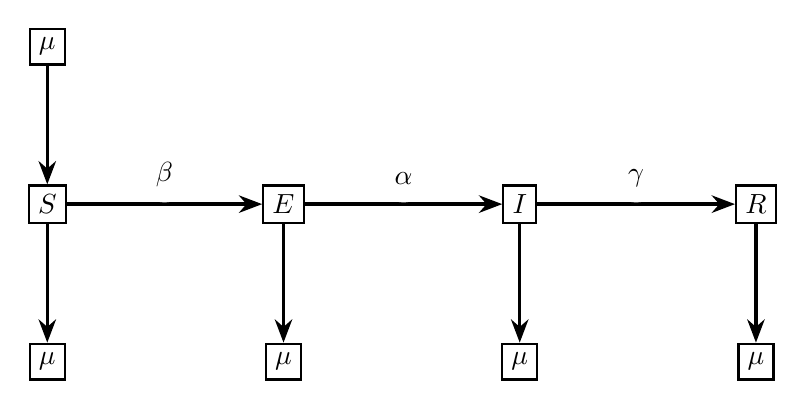
\begin{tikzpicture}[scale=2]
		\begin{scope}[every node/.style={thick,draw}]
			\node (births) at (0,1) {$\mu$};
			\node (S) at (0,0) {$S$};
			\node (deaths1) at (0,-1) {$\mu$};
			\node (E) at (1.5,0) {$E$};
			\node (deaths2) at (1.5,-1) {$\mu$};
			\node (I) at (3,0) {$I$};
			\node (deaths3) at (3,-1) {$\mu$};
			\node (R) at (4.5,0) {$R$};
			\node (deaths4) at (4.5,-1) {$\mu$};
		\end{scope}
		\begin{scope}[>={Stealth[black]},
			every node/.style={fill=white,circle},
			every edge/.style={draw=black,very thick}]
			\path [->] (births) edge (S);
			\path [->] (S) edge node[above] {$\beta$} (E);
			\path [->] (S) edge (deaths1);
			\path [->] (E) edge node[above] {$\alpha$} (I);
			\path [->] (E) edge (deaths2);
			\path [->] (I) edge node[above] {$\gamma$} (R);
			\path [->] (I) edge (deaths3);
			\path [->] (R) edge (deaths4);
		\end{scope}
	\end{tikzpicture}
	\caption{SEIR Model with Vital Statistics}
	\label{fig:seir-model-statistics}
\end{figure}

\begin{equation*}
\begin{aligned}
	S' &= \mu - \mu S - \beta I S\\
	&= 0\\
	E' &= \beta I S - (\mu + \alpha) E\\
	&= 0\\
	I &= \alpha E - (\mu + \gamma) I\\
	&= 0
\end{aligned}
\end{equation*}

Guess:
\begin{equation*}
\begin{aligned}
	I^{*} &= 0\\
	&\Rightarrow S^{*} = 1\\
	&\Rightarrow E^{*} = 0\\
\end{aligned}
\end{equation*}

Null clines:
\begin{equation*}
\begin{aligned}
	S' = 0 \sep I &= \frac{\mu}{\beta}\left( \frac{1}{S} - 1 \right)\\
	E' = 0 \sep E &= \frac{\beta}{\mu + \alpha}SI\\
	I' = 0 \sep E &= \frac{\mu + \gamma}{\alpha} I\\
\end{aligned}
\end{equation*}
\begin{equation*}
\begin{aligned}
	E' &= I'\\
	\frac{\beta}{\mu + \alpha}SI &= \frac{\mu + \gamma}{\alpha} I\\
	\frac{\beta}{\mu + \alpha}S &= \frac{\mu + \gamma}{\alpha}\\
	S_{2}^{*} &= \frac{\mu + \alpha}{\beta}\frac{\mu + \gamma}{\alpha}\\
			  &= \frac{(\mu + \alpha)(\mu + \gamma)}{\beta\alpha}\\
	I_{2}^{*} &= \frac{\mu\alpha}{(\mu + \gamma)(\mu + \alpha)} - \frac{\mu}{\beta}\\
	E_{2}^{*} &= \frac{\mu + \gamma}{\alpha}I_{2}^{*}\\
			  &= \frac{\mu + \gamma}{\alpha}\left( \frac{\mu\alpha}{(\mu + \gamma)(\mu + \alpha)} - \frac{\mu}{\beta} \right)\\
			  &= \frac{\mu}{\mu + \alpha} - \frac{\mu(\mu + \gamma)}{\beta\alpha}\\
\end{aligned}
\end{equation*}

When is $Q_{2}^{*}$ in the domain?



\begin{equation*}
\begin{aligned}
	E_{2}^{*} &= \frac{\mu}{\mu + \gamma}\left[ 1 - \frac{1}{R_{0}} \right]
\end{aligned}
\end{equation*}

Obtain $R_{0}$ without math above
Claim:
\begin{equation*}
\begin{aligned}
	R_{0} &= \left( \mbox{number of contacts per unit time} \right)\left( \mbox{probability of transmission per coontact} \right) \\&\times \left( \mbox{duration of infection} \right)\left( \mbox{probability of surviving} \right)\\
	&= \left( \beta \right)\left( 1 \right)\left( \frac{1}{\gamma + \mu} \right)\left( \frac{\alpha}{\alpha + \mu} \right)
\end{aligned}
\end{equation*}

\section{How do vaccinations affect the models?}\label{sec:how-do-vaccinations-affect-the-models?}

\begin{figure}[H]
	\centering
	\begin{tikzpicture}[scale=2]
		\begin{scope}[every node/.style={thick,draw}]
			\node (births) at (0,1) {$d$};
			\node (S) at (0,0) {$S$};
			\node (deaths1) at (0,-1) {$d$};
			\node (I) at (1.5,0) {$I$};
			\node (deaths2) at (1.5,-1) {$d$};
			\node (R) at (3,0) {$R$};
			\node (deaths3) at (3,-1) {$d$};
		\end{scope}
		\begin{scope}[>={Stealth[black]},
			every node/.style={fill=white,circle},
			every edge/.style={draw=black,very thick}]
			\path [->] (births) edge (S);
			\path [->] (S) edge node[above] {$\beta$} (E);
			\path [->] (S) edge (deaths1);
			\path [->] (I) edge node[above] {$\mu$} (R);
			\path [->] (I) edge (deaths2);
			\path [->] (R) edge (deaths3);
			\path [->] (S) edge[bend left=45] node[above] {$V$} (R);
		\end{scope}
	\end{tikzpicture}
	\caption{SEIR Model with Vital Statistics}
	\label{fig:seir-model-statistics-vaccines}
\end{figure}

If $V$ is large enough: $I^{*}$ go negative

\section{Artificial Inteliigence (AI)}\label{sec:artificial-inteliigence-(ai)}
ML - Machine Learning
DL - Deep Learning


\end{document}